\documentclass[paper=letter,11pt]{scrartcl}

\KOMAoptions{headinclude=true, footinclude=false}
\KOMAoptions{DIV=14, BCOR=5mm}
\KOMAoptions{numbers=noendperiod}
\KOMAoptions{parskip=half}
\addtokomafont{disposition}{\rmfamily}
\addtokomafont{part}{\LARGE}
\addtokomafont{descriptionlabel}{\rmfamily}
%\setkomafont{pageheadfoot}{\normalsize\sffamily}
\setkomafont{pagehead}{\normalsize\rmfamily}
%\setkomafont{publishers}{\normalsize\rmfamily}
\setkomafont{caption}{\normalfont\small}
\setcapindent{0pt}
\deffootnote[1em]{1em}{1em}{\textsuperscript{\thefootnotemark}\ }


\usepackage{amsmath}
\usepackage[varg]{txfonts}
\usepackage[T1]{fontenc}
\usepackage{graphicx}
\usepackage{xcolor}
\usepackage[american]{babel}
% hyperref is needed in many places, so include it here
\usepackage{hyperref}

\usepackage{xspace}
\usepackage{multirow}
\usepackage{float}


\usepackage{braket}
\usepackage{bbm}
\usepackage{relsize}
\usepackage{tcolorbox}

\def\ketY{\ensuremath{\ket {\Psi}}}
\def\iGeV{\ensuremath{\textrm{GeV}^{-1}}}
%\def\mp{\ensuremath{m_{\textrm{proton}}}}
\def\rp{\ensuremath{r_{\textrm{proton}}}}
\def\me{\ensuremath{m_{\textrm{electron}}}}
\def\aG{\ensuremath{\alpha_G}}
\def\rAtom{\ensuremath{r_{\textrm{atom}}}}
\def\rNucl{\ensuremath{r_{\textrm{nucleus}}}}
\def\GN{\ensuremath{\textrm{G}_\textrm{N}}}
\def\ketX{\ensuremath{\ket{\vec{x}}}}
\def\ve{\ensuremath{\vec{\epsilon}}}


\def\ABCDMatrix{\ensuremath{\begin{pmatrix} A &  B  \\ C  & D \end{pmatrix}}}
\def\xyprime{\ensuremath{\begin{pmatrix} x' \\ y' \end{pmatrix}}}
\def\xyprimeT{\ensuremath{\begin{pmatrix} x' &  y' \end{pmatrix}}}
\def\xy{\ensuremath{\begin{pmatrix} x \\ y \end{pmatrix}}}
\def\xyT{\ensuremath{\begin{pmatrix} x & y \end{pmatrix}}}

\def\IMatrix{\ensuremath{\begin{pmatrix} 0 &  1  \\ -1  & 0 \end{pmatrix}}}
\def\IBoostMatrix{\ensuremath{\begin{pmatrix} 0 &  1  \\ 1  & 0 \end{pmatrix}}}
\def\JThree{\ensuremath{\begin{pmatrix}    0 & -i & 0  \\ i & 0  & 0 \\ 0 & 0 & 0 \end{pmatrix}}} 
\def\JTwo{\ensuremath{\begin{bmatrix}    0 & 0 & -i  \\ 0 & 0  & 0 \\ i & 0 & 0 \end{bmatrix}}}
\def\JOne{\ensuremath{\begin{bmatrix}    0 & 0 & 0  \\ 0 & 0  & -i \\ 0 & i & 0 \end{bmatrix}}}
\def\etamn{\ensuremath{\eta_{\mu\nu}}}
\def\Lmn{\ensuremath{\Lambda^\mu_\nu}}
\def\dmn{\ensuremath{\delta^\mu_\nu}}
\def\wmn{\ensuremath{\omega^\mu_\nu}}
\def\be{\begin{equation*}}
\def\ee{\end{equation*}}
\def\bea{\begin{eqnarray*}}
\def\eea{\end{eqnarray*}}
\def\bi{\begin{itemize}}
\def\ei{\end{itemize}}
\def\fmn{\ensuremath{F_{\mu\nu}}}
\def\fMN{\ensuremath{F^{\mu\nu}}}
\def\bc{\begin{center}}
\def\ec{\end{center}}
\def\nus{$\nu$s}

\def\adagger{\ensuremath{a_{p\sigma}^\dagger}}
\def\lineacross{\noindent\rule{\textwidth}{1pt}}

\newcommand{\multiline}[1] {
\begin{tabular} {|l}
#1
\end{tabular}
}

\newcommand{\multilineNoLine}[1] {
\begin{tabular} {l}
#1
\end{tabular}
}



\newcommand{\lineTwo}[2] {
\begin{tabular} {|l}
#1 \\
#2
\end{tabular}
}

\newcommand{\rmt}[1] {
\textrm{#1}
}


%
% Units
%
\def\m{\ensuremath{\rmt{m}}}
\def\GeV{\ensuremath{\rmt{GeV}}}
\def\pt{\ensuremath{p_\rmt{T}}}


\def\parity{\ensuremath{\mathcal{P}}}

\usepackage{cancel}
\usepackage{ mathrsfs }
\def\bigL{\ensuremath{\mathscr{L}}}

\usepackage{ dsfont }



\usepackage{fancyhdr}
\fancyhf{}

%\documentclass[margin,line]{res}
\usepackage{braket}
\usepackage{bbm}
\usepackage{relsize}
\usepackage{tcolorbox}


\def\ketY{\ensuremath{\ket {\Psi}}}
\def\iGeV{\ensuremath{\textrm{GeV}^{-1}}}
%\def\mp{\ensuremath{m_{\textrm{proton}}}}
\def\rp{\ensuremath{r_{\textrm{proton}}}}
\def\me{\ensuremath{m_{\textrm{electron}}}}
\def\aG{\ensuremath{\alpha_G}}
\def\rAtom{\ensuremath{r_{\textrm{atom}}}}
\def\rNucl{\ensuremath{r_{\textrm{nucleus}}}}
\def\GN{\ensuremath{\textrm{G}_\textrm{N}}}
\def\ketX{\ensuremath{\ket{\vec{x}}}}
\def\ve{\ensuremath{\vec{\epsilon}}}


\def\ABCDMatrix{\ensuremath{\begin{pmatrix} A &  B  \\ C  & D \end{pmatrix}}}
\def\xyprime{\ensuremath{\begin{pmatrix} x' \\ y' \end{pmatrix}}}
\def\xyprimeT{\ensuremath{\begin{pmatrix} x' &  y' \end{pmatrix}}}
\def\xy{\ensuremath{\begin{pmatrix} x \\ y \end{pmatrix}}}
\def\xyT{\ensuremath{\begin{pmatrix} x & y \end{pmatrix}}}

\def\IMatrix{\ensuremath{\begin{pmatrix} 0 &  1  \\ -1  & 0 \end{pmatrix}}}
\def\IBoostMatrix{\ensuremath{\begin{pmatrix} 0 &  1  \\ 1  & 0 \end{pmatrix}}}
\def\JThree{\ensuremath{\begin{pmatrix}    0 & -i & 0  \\ i & 0  & 0 \\ 0 & 0 & 0 \end{pmatrix}}} 
\def\JTwo{\ensuremath{\begin{bmatrix}    0 & 0 & -i  \\ 0 & 0  & 0 \\ i & 0 & 0 \end{bmatrix}}}
\def\JOne{\ensuremath{\begin{bmatrix}    0 & 0 & 0  \\ 0 & 0  & -i \\ 0 & i & 0 \end{bmatrix}}}
\def\etamn{\ensuremath{\eta_{\mu\nu}}}
\def\Lmn{\ensuremath{\Lambda^\mu_\nu}}
\def\dmn{\ensuremath{\delta^\mu_\nu}}
\def\wmn{\ensuremath{\omega^\mu_\nu}}
\def\be{\begin{equation*}}
\def\ee{\end{equation*}}
\def\bea{\begin{eqnarray*}}
\def\eea{\end{eqnarray*}}
\def\bi{\begin{itemize}}
\def\ei{\end{itemize}}
\def\fmn{\ensuremath{F_{\mu\nu}}}
\def\fMN{\ensuremath{F^{\mu\nu}}}
\def\bc{\begin{center}}
\def\ec{\end{center}}
\def\nus{$\nu$s}

\def\adagger{\ensuremath{a_{p\sigma}^\dagger}}
\def\lineacross{\noindent\rule{\textwidth}{1pt}}

\newcommand{\multiline}[1] {
\begin{tabular} {|l}
#1
\end{tabular}
}

\newcommand{\multilineNoLine}[1] {
\begin{tabular} {l}
#1
\end{tabular}
}



\newcommand{\lineTwo}[2] {
\begin{tabular} {|l}
#1 \\
#2
\end{tabular}
}

\newcommand{\rmt}[1] {
\textrm{#1}
}


%
% Units
%
\def\m{\ensuremath{\rmt{m}}}
\def\GeV{\ensuremath{\rmt{GeV}}}
\def\pt{\ensuremath{p_\rmt{T}}}


\def\parity{\ensuremath{\mathcal{P}}}

\usepackage{cancel}
\usepackage{ mathrsfs }
\def\bigL{\ensuremath{\mathscr{L}}}

\usepackage{ dsfont }


\usepackage{cancel}

\usepackage{fancyhdr}

\fancyhf{}
\lhead{\Large 33-444} % \hfill Introduction to Particle Physics \hfill Spring 2020}
\chead{\Large Introduction to Particle Physics} % \hfill Spring 2020}
\rhead{\Large Spring 2020} % \hfill Introduction to Particle Physics \hfill Spring 2020}

\begin{document}
\thispagestyle{fancy}

\begin{center}
{\huge \textbf{Lecture 18}}
\end{center}

{\fontsize{14}{16}\selectfont

\underline{Now do the same thing to a more general interaction}


\begin{figure}[h]
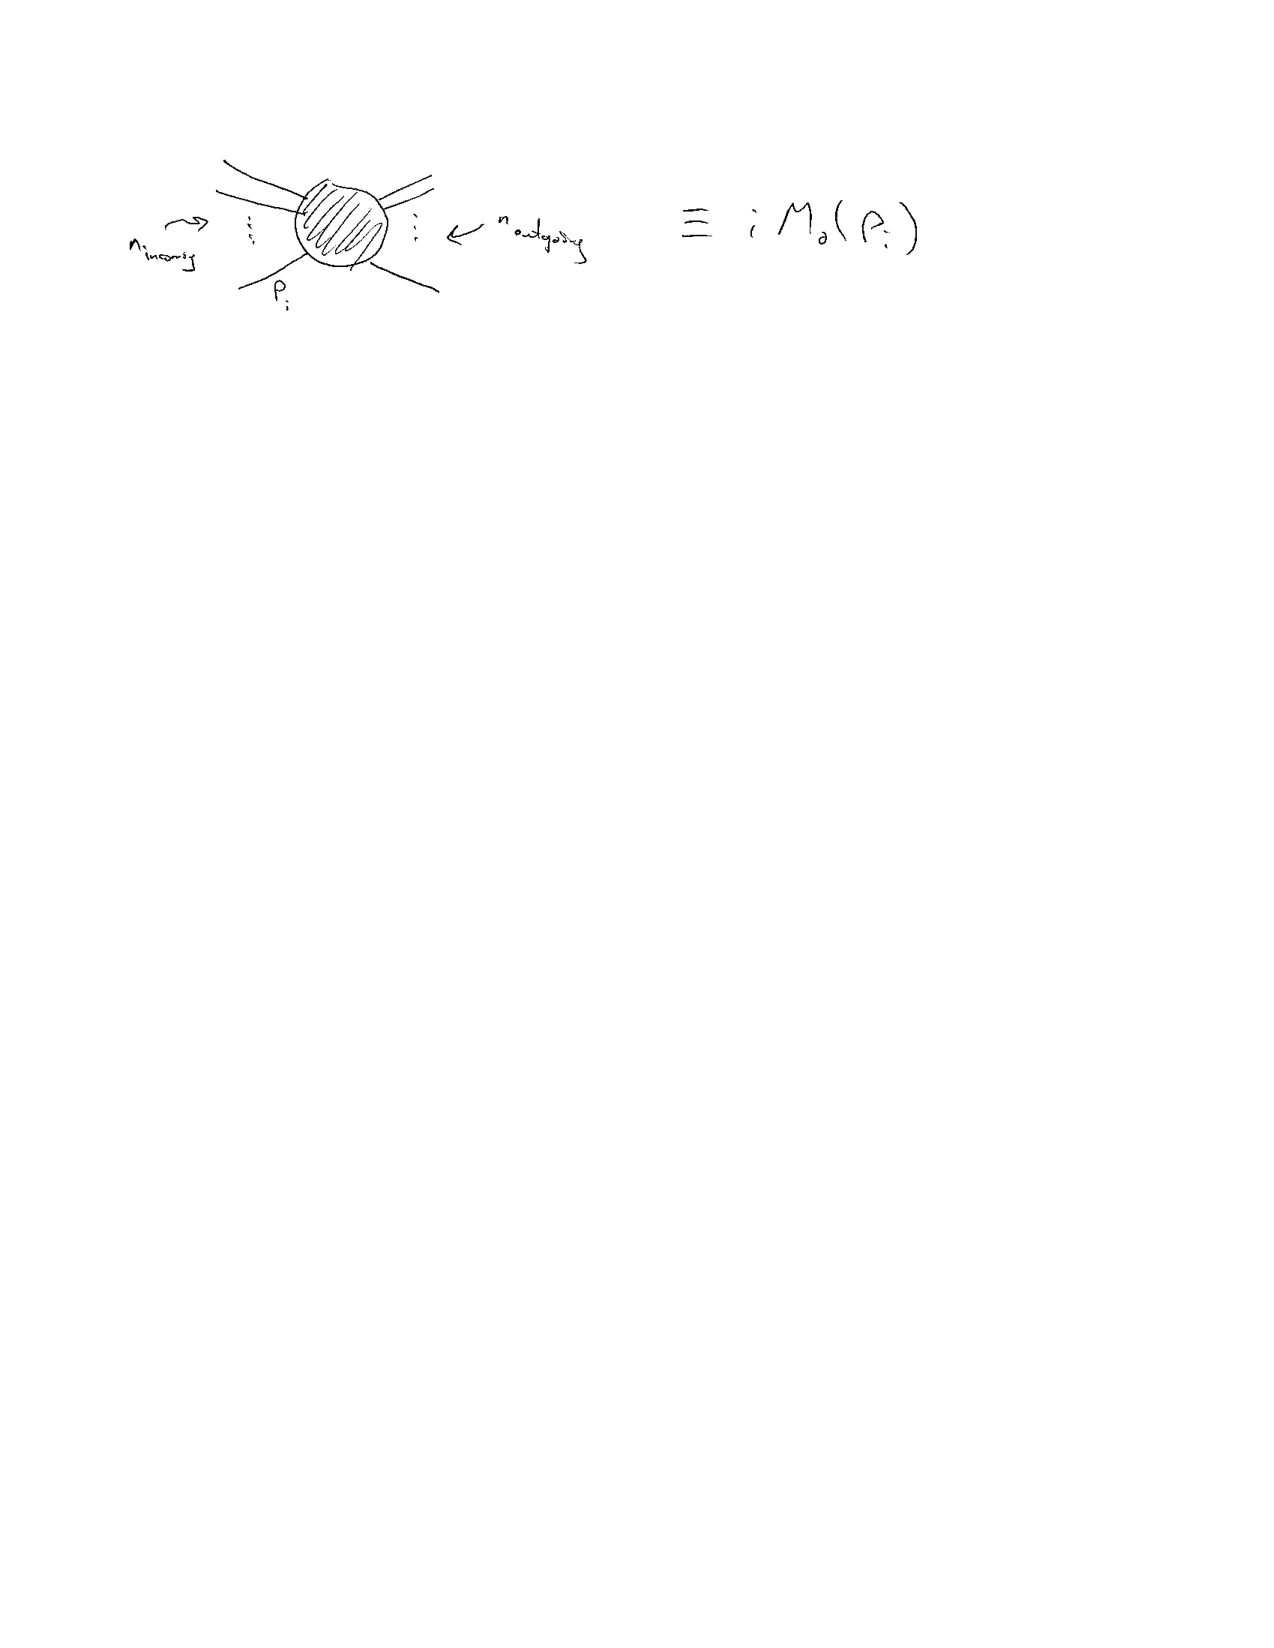
\includegraphics[width=0.99\textwidth]{./generalScattering.pdf}
\end{figure}

Consider what happens if we attach a ``photon'' to an incoming leg

\begin{figure}[h]
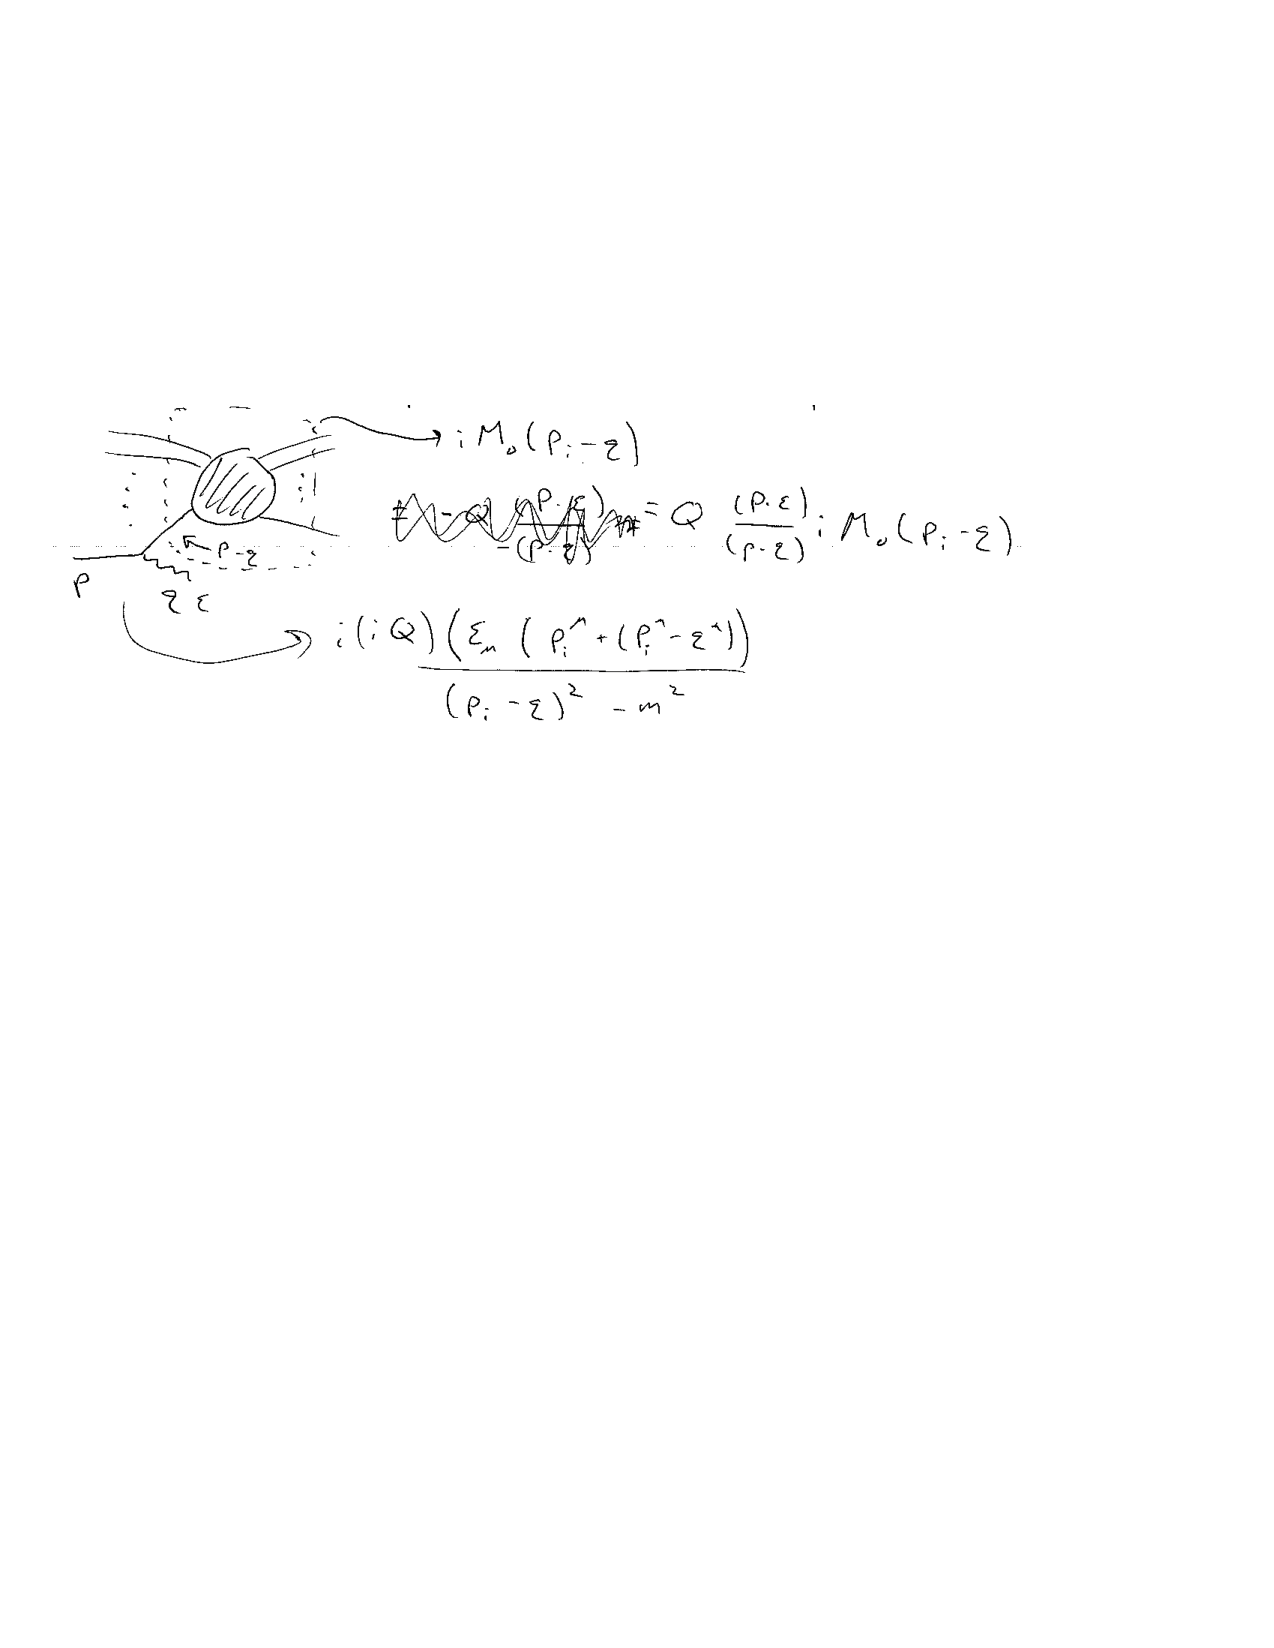
\includegraphics[width=0.99\textwidth]{./incomingPhoton.pdf}
\end{figure}

\clearpage

Can also attach photon to outgoing leg

\begin{figure}[h]
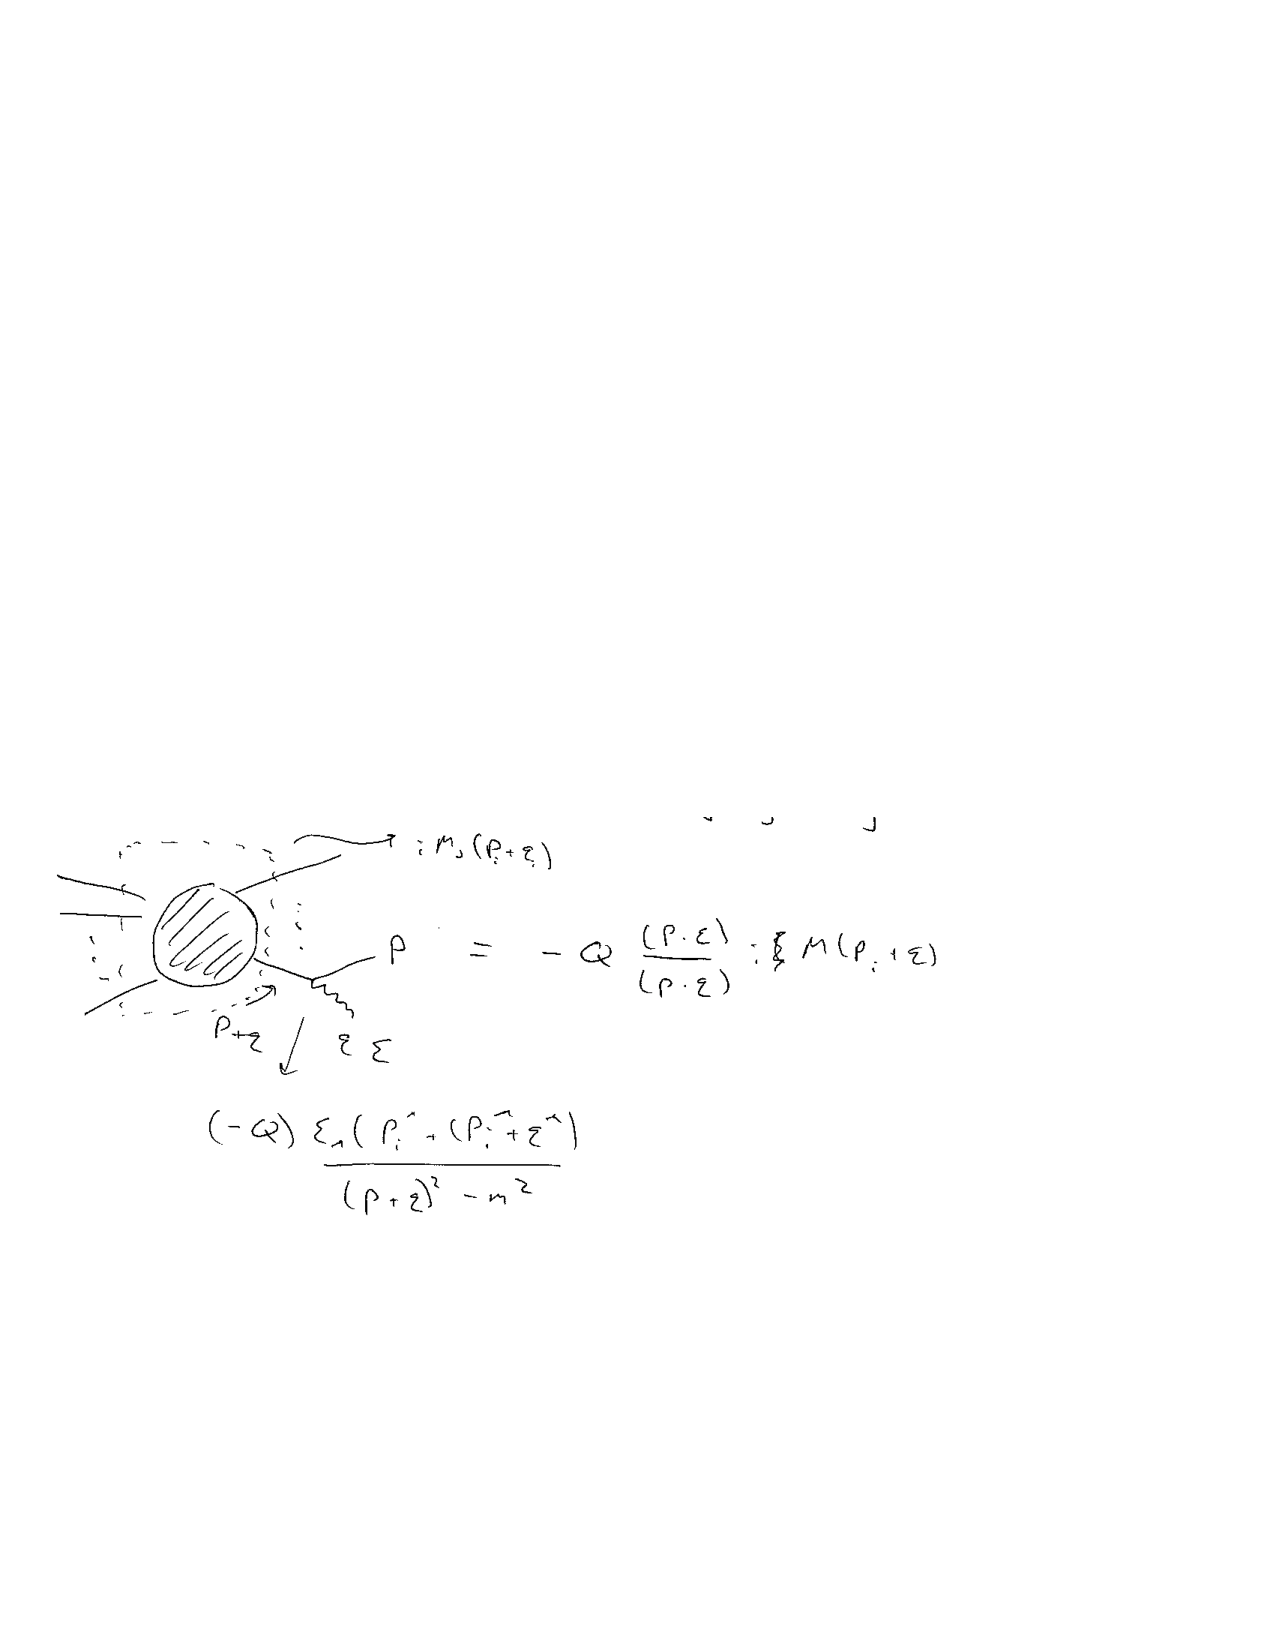
\includegraphics[width=0.99\textwidth]{./outgoingPhoton.pdf}
\end{figure}

Total Amplitude is then given by

\be
M  = \sum_{\rmt{incoming}} Q_i \frac{(p\cdot\epsilon)}{(p\cdot q)}\ i M_0(p-q) + \sum_{\rmt{outgoing}} - Q_i \frac{(p\cdot\epsilon)}{(p\cdot q)}\ i M_0(p+q)
\ee

Take soft limit: $M_0(p\pm q) \rightarrow M_0(p)$

\be
M  = iM_0 \left( \sum_{\rmt{incoming}} Q_i \frac{(p\cdot\epsilon)}{(p\cdot q)}\  + \sum_{\rmt{outgoing}} - Q_i \frac{(p\cdot\epsilon)}{(p\cdot q)}\   \right)
\ee

Now as before $\epsilon_\mu \rightarrow \epsilon'_\mu + q_\mu$ means that M must vanish when $\epsilon_\mu \rightarrow q_\mu$.

OR under a Lorentz Transform

\be
\epsilon_\mu \cdot M \rightarrow \epsilon'_\mu \cdot M' + i M_0 \underbrace{\left( \sum_{\rmt{incoming}} Q_i  + \sum_{\rmt{outgoing}} - Q_i    \right)}_{\substack{= 0\ \rmt{only if} \\ \sum_{\rmt{incoming}} Q_i = \sum_{\rmt{outgoing}} Q_i }}
\ee

\underline{\underline{Charge has to be conserved! }}

\lineacross

Now same logic for Spin-2  (describes interaction w/Gravitons)

Same as above except 2-component polarization vector.


\be
\epsilon_{\mu\nu} \underbrace{\rightarrow}_{\rmt{under little group}} \epsilon_{\mu\nu} + \underbrace{A_\mu q_\nu + B_\mu q_\mu + C q_\mu q_\nu}_{\rmt{effect from all of these need to be 0 as before}}
\ee

where A, B C's are non-zero and depend on the particular little group transformation done.


\begin{minipage}{0.4\textwidth}
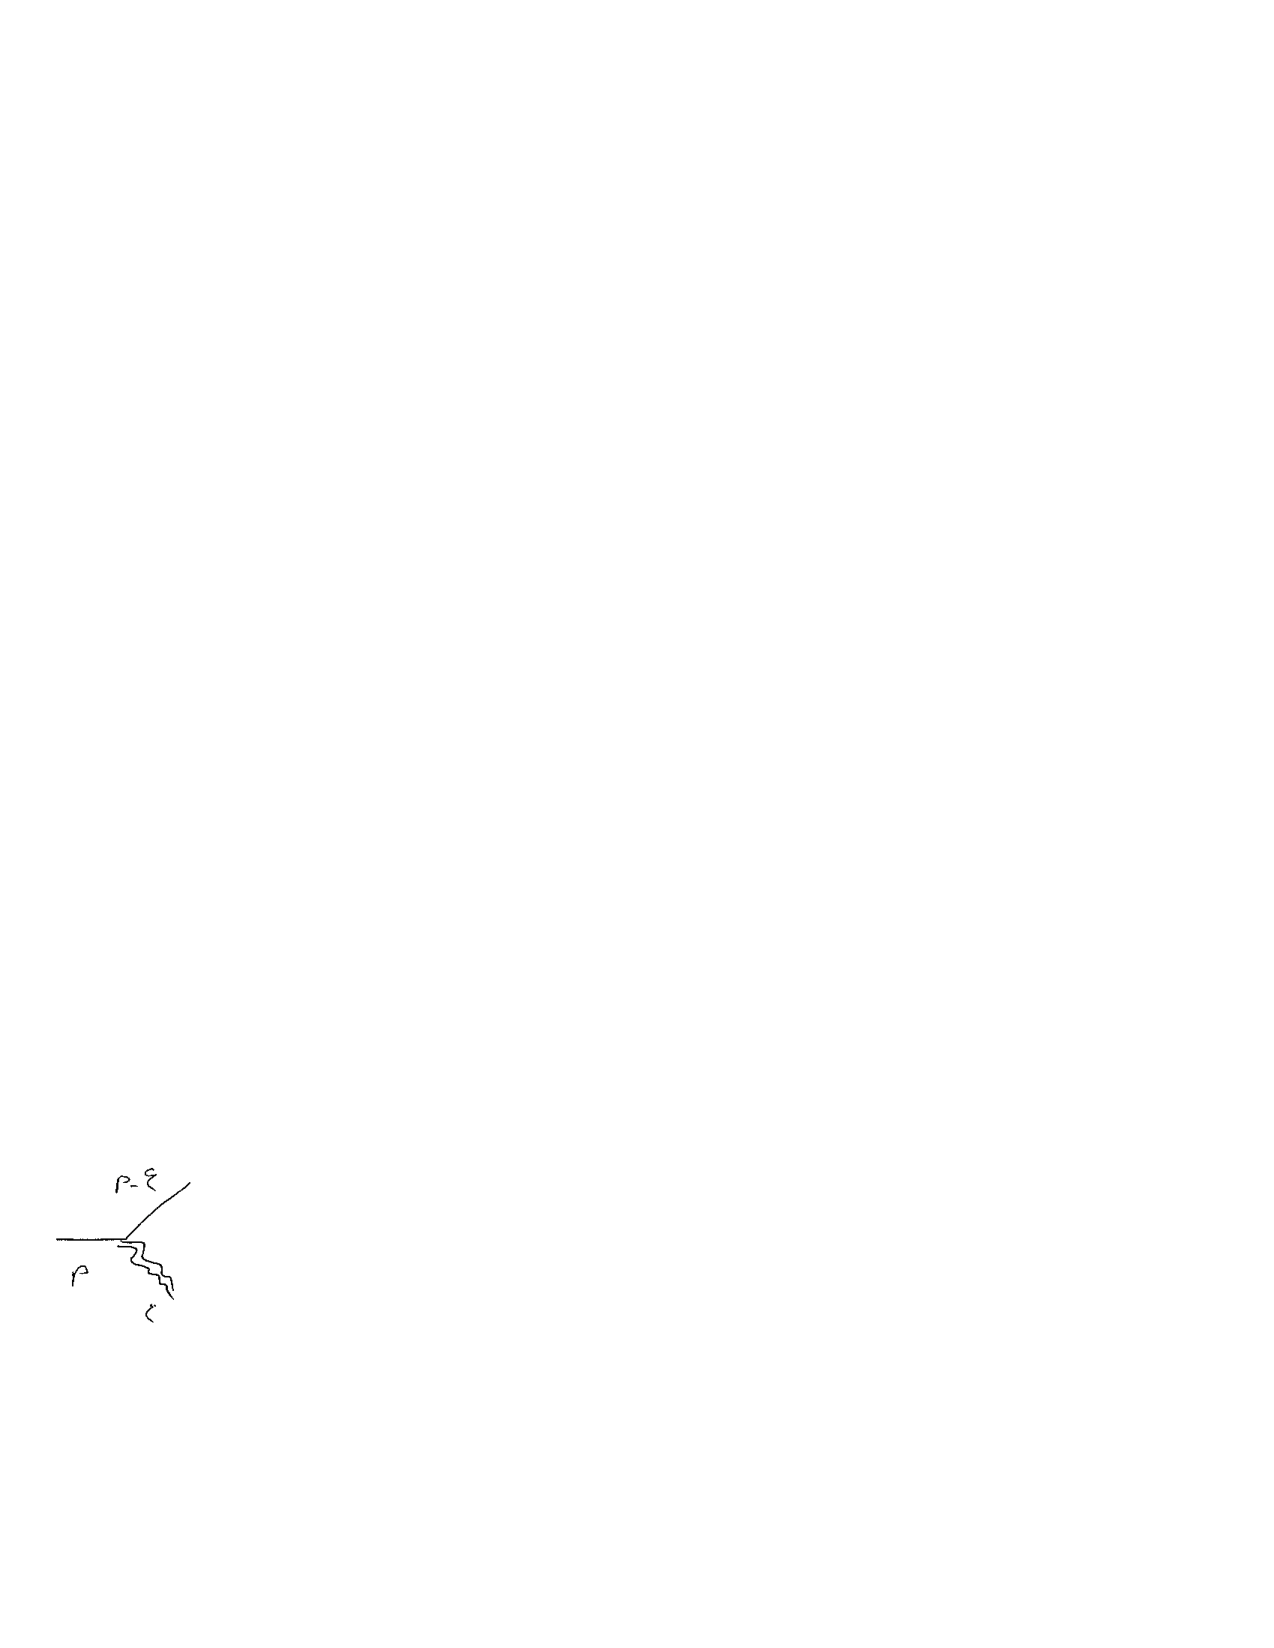
\includegraphics[width=0.9\textwidth]{./gravitonVertex.pdf}
\end{minipage} %\hfill
\begin{minipage}{0.45\textwidth}
\be
= i (iK_i) \epsilon_{\mu\nu} \frac{(2p^\mu p^\nu)}{-p\cdot q}
\ee
\end{minipage} %\hfill

(Same idea with the outgoing leg)


Now, (lets focus on piece that goes like $\epsilon_{\mu\nu} \rightarrow  \epsilon_{\mu\nu}  + q_\mu B_\nu$

\bea
\epsilon_{\mu\nu} \rightarrow  \epsilon'_{\mu\nu} M'^{\mu\nu} &+& M \left( \sum_{\rmt{incoming}} K_i B_\nu p^\nu - \sum_{\rmt{outgoing}} K_i B_\nu p^\nu \right)\\
&+& M B_\nu \left( \sum_{\rmt{incoming}} K_i  p^\nu - \sum_{\rmt{outgoing}} K_i  p^\nu \right)
\eea

$\Rightarrow  K_i p_i^\nu$  is \underline{\underline{conserved}}


We know that $p_i^\nu$ is conserved by E and momentum conservation. 

Only way can have nontrivial solutions is if $k_i = k$ for all i

All particles interact with gravity with the same strength. 

\underline{Gravitational interaction is Universal !}

Discovered the ``Principle of Equivalence'' that is the starting point of General Relativity!

\lineacross

Can keep going...

For a massless spin-3 particle we would do the same exercise. 

We would find we need

\be
 \sum_{\rmt{incoming}} \beta_i  p_i^\mu p_i^\nu = \sum_{\rmt{outgoing}} \beta_i  p_i^\mu  p_i^\nu 
\ee

eg: $\mu\nu = 0$

\be
 \sum_{\rmt{incoming}} \beta_i  E_i^2 = \sum_{\rmt{outgoing}} \beta_i  E_i^2
\ee


Way too constraining.  

Only way if $\beta_i = 0$

\underline{\underline{There can be no interacting theories of massless particles of Spin greater than 2 !}}


}
\end{document}

